\section{Results}
\label{sec:results}

Each result is labelled \emph{strong}, \emph{weak} or \emph{null} against its pre-registered criterion; the verdict opens each subsection.

\subsection{Speaker Attribution}
\emph{Verdict: null against the gate.}

On 330 driver/engineer-labelled turns, the primary system reaches \textbf{0.670} accuracy (95\% CI 0.610--0.726; season-reweighted 0.682), well below the 0.85 gate (Fig.~\ref{fig:attr}). When it predicts \textsc{driver} it is right 65\% of the time; it recovers 56\% of true driver turns. The brief's literal two-cluster-per-channel variant is at chance (0.515), voice alone gives 0.646 and text cues alone 0.391: \emph{language cannot tell driver from engineer here; voice can, partially.} Accuracy degrades from 0.72--0.77 (2018--2021) to 0.51 in 2025. Diarization is not the main failure (only 4.4\% of labelled turns contained both speakers); naming which voice cluster is the driver is. Test--retest agreement on 20 repeated items was 0.90. An independent check came from Stage~C: 30\% (133/450) of utterances sampled as \textsc{driver} were flagged by the annotator as not the driver. We therefore proceeded only with \emph{human-verified} driver utterances for T1--T3, a logged deviation from the brief's instruction to stop.

\begin{figure}[t]
\centering
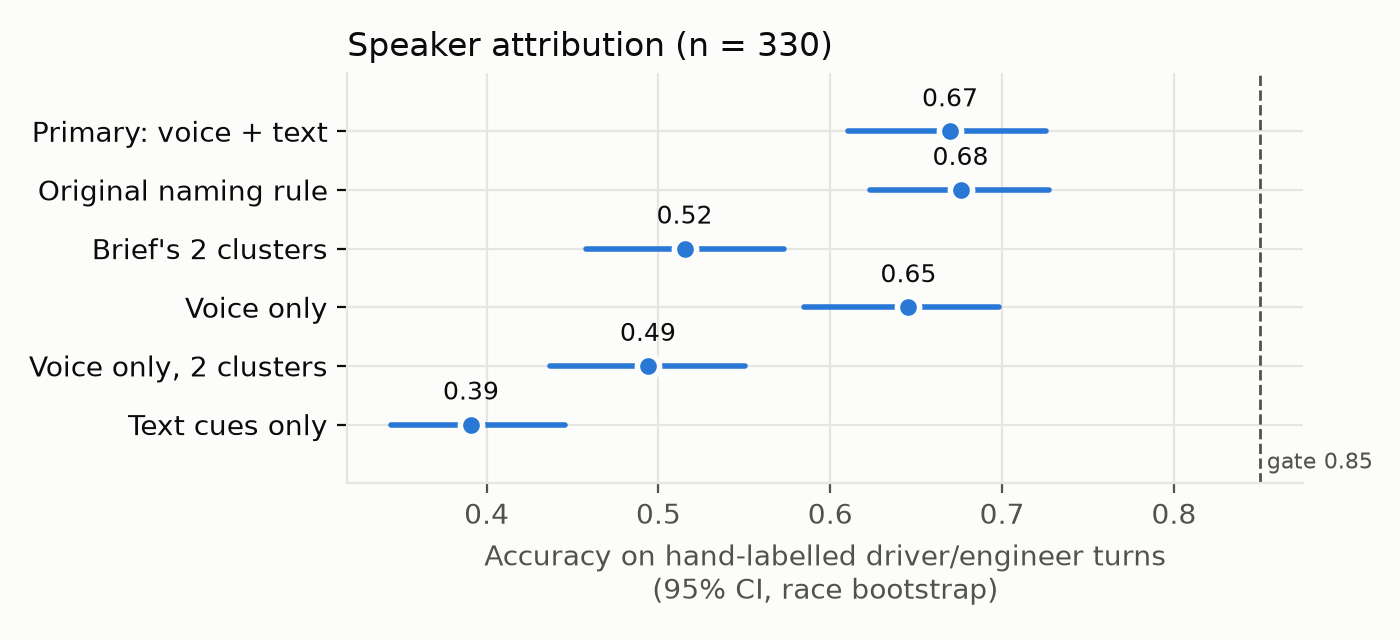
\includegraphics[width=\columnwidth]{fig1_attribution.png}
\caption{Speaker-attribution accuracy with race-bootstrap 95\% CIs; dashed line: pre-registered gate.}
\label{fig:attr}
\end{figure}

\subsection{Word Error Rate with Prompting}
\emph{Verdict: weak.}

On 41 hand-transcribed clips (859 words), WER is 0.298 for the dataset's transcripts, 0.302 for plain Whisper large-v3 and 0.290 with season-specific prompting: a 2.7\% relative reduction against the dataset (paired 95\% CI $-3.2$\% to $+7.6$\%) and 3.8\% against plain Whisper, far below the 15\% adoption bar. Downstream stages therefore keep the unprompted transcripts. Transcription errors visibly propagate (e.g.\ ``Enjoy one more tea guys'' in a misclassified utterance).

\subsection{Lap-Time Model}
\emph{Verdict: strong.}

Across 147 races and 139{,}995 clean laps, held-out RMSE is 0.70\,s per lap (median race; IQR 0.59--0.88; MAE 0.48), against 1.12\,s for a per-driver mean, explaining 75\% of lap-time variance. The fuel-burn slope, $-0.057$\,s/lap, has the expected sign and magnitude. All T2 and T4 analyses inherit this 0.7\,s noise floor.

\subsection{Annotation Statistics}
Of 450 labelled utterances, 317 were the driver (250 in-race): \textsc{no\_claim} 123, \textsc{grip\_deg} 49, \textsc{no\_sensor} 45, \textsc{rel\_pace} 32, \textsc{incident} 32, \textsc{traffic} 25, \textsc{power} 11; arousal low/mid/high 158/126/33. Under the brief's 100-instance rule only \textsc{no\_claim} would survive, so we use the threshold of 30 stated before labelling (five classes; \textsc{traffic} and \textsc{power} are dropped and reported in a sensitivity analysis). With one annotator, no inter-annotator $\kappa$~\cite{cohen1960kappa} can be computed; this is a central limitation. The 2025 test season contains only 37 driver items, so race-grouped CV is the headline.

\subsection{Claim-Type Classification (T1)}
\emph{Verdict: strong.}

\begin{table}[t]
\centering
\caption{T1 claim type and T3 text arousal, 5-fold race-grouped CV. Macro AUC-PR [95\% CI]. Chance = mean AUC-PR of random rankings of the same labels.}
\label{tab:t1}
\begin{tabular}{lcc}
\toprule
Model & Claim type (5 classes) & Arousal (3 levels) \\
\midrule
Chance & 0.215 & 0.344 \\
Majority & 0.179 & 0.309 \\
Context only (no text) & 0.320 [0.282, 0.378] & 0.400 [0.371, 0.450] \\
TF-IDF + LR & \textbf{0.466} [0.422, 0.528] & 0.487 [0.429, 0.556] \\
DeBERTa-v3 (multi-task) & 0.426 [0.385, 0.496] & \textbf{0.544} [0.485, 0.618] \\
\midrule
LLM zero-shot (no training) & \textbf{0.629} [0.578, 0.691] & -- \\
\bottomrule
\end{tabular}
\end{table}
Table~\ref{tab:t1} gives the headline. The fine-tuned DeBERTa beats the context-only baseline by $+0.106$ macro AUC-PR (paired 95\% CI $+0.039$ to $+0.179$), so the words carry claim information beyond race context. It does not beat TF-IDF (0.426 vs.\ 0.466): with $\sim$250 training examples per fold, a 184M-parameter encoder does not overtake lexical features. Per class (Fig.~\ref{fig:conf}), TF-IDF is much stronger on \textsc{grip\_deg} (0.72 vs.\ 0.49) and \textsc{incident} (0.54 vs.\ 0.30), which have distinctive keywords (``grip'', ``contact'', ``penalty''); DeBERTa is stronger on \textsc{no\_claim} (0.77 vs.\ 0.63) and \textsc{rel\_pace} (0.28 vs.\ 0.18). DeBERTa's main confusions are semantic and taxonomic: incidents described as another driver's behaviour are read as relative pace (16 of 32), and car-feel complaints that public telemetry cannot check (\textsc{no\_sensor}, e.g.\ brakes) are read as tyre grip (24 of 45). For arousal, the multi-task DeBERTa is the best text model (0.544; $+0.144$ over context, CI $+0.061$ to $+0.218$).

\textbf{A zero-shot LLM beats both trained models.} Given only the category definitions from the annotation guide, Qwen2.5-1.5B-Instruct reaches 0.629 macro AUC-PR (CI 0.578--0.691; argmax accuracy 0.62) with no training. On the same 281 items it beats the fine-tuned DeBERTa by $+0.203$ (paired CI $+0.118$ to $+0.271$) and TF-IDF by $+0.164$ ($+0.088$ to $+0.230$). Its largest gains are on the classes the trained models found hardest, \textsc{incident} (0.74) and \textsc{no\_sensor} (0.56). Because the LLM sees no labels, leakage is impossible. Its advantage is the information in the definitions themselves, which the trained models had to infer from $\sim$250 examples.

\textbf{Other splits.} The result holds on every split (Table~\ref{tab:splits}). On the 2025 test season, used once, DeBERTa beats context-only by $+0.187$ (CI $+0.073$ to $+0.381$) despite only 37 items. Under leave-one-driver-out, performance on unseen drivers (0.475) is no lower than under race-grouped CV, so the model learned claim language rather than driver identity. DeBERTa versus TF-IDF has no consistent winner: TF-IDF leads in CV, DeBERTa on the 2024, 2025 and LODO splits. Lowering the class threshold to 20 (adding \textsc{traffic}, six classes) leaves the conclusion unchanged: DeBERTa beats context by $+0.105$ (CI $+0.055$ to $+0.158$), while \textsc{traffic} itself is barely above chance (0.11 vs.\ 0.10).

\begin{table}[t]
\centering
\caption{T1 claim type, macro AUC-PR on each split. Chance is the 95th percentile of random rankings.}
\label{tab:splits}
\begin{tabular}{lcccc}
\toprule
Split & DeBERTa & TF-IDF & Context & Chance$_{95}$ \\
\midrule
Race-grouped CV & 0.426 & \textbf{0.466} & 0.320 & 0.237 \\
Val.\ 2024 & \textbf{0.481} & 0.461 & 0.286 & 0.347 \\
Test 2025 & \textbf{0.468} & 0.394 & 0.281 & 0.415 \\
Leave-one-driver-out & \textbf{0.475} & 0.455 & -- & 0.255 \\
\bottomrule
\end{tabular}
\end{table}

\begin{figure*}[t]
\centering
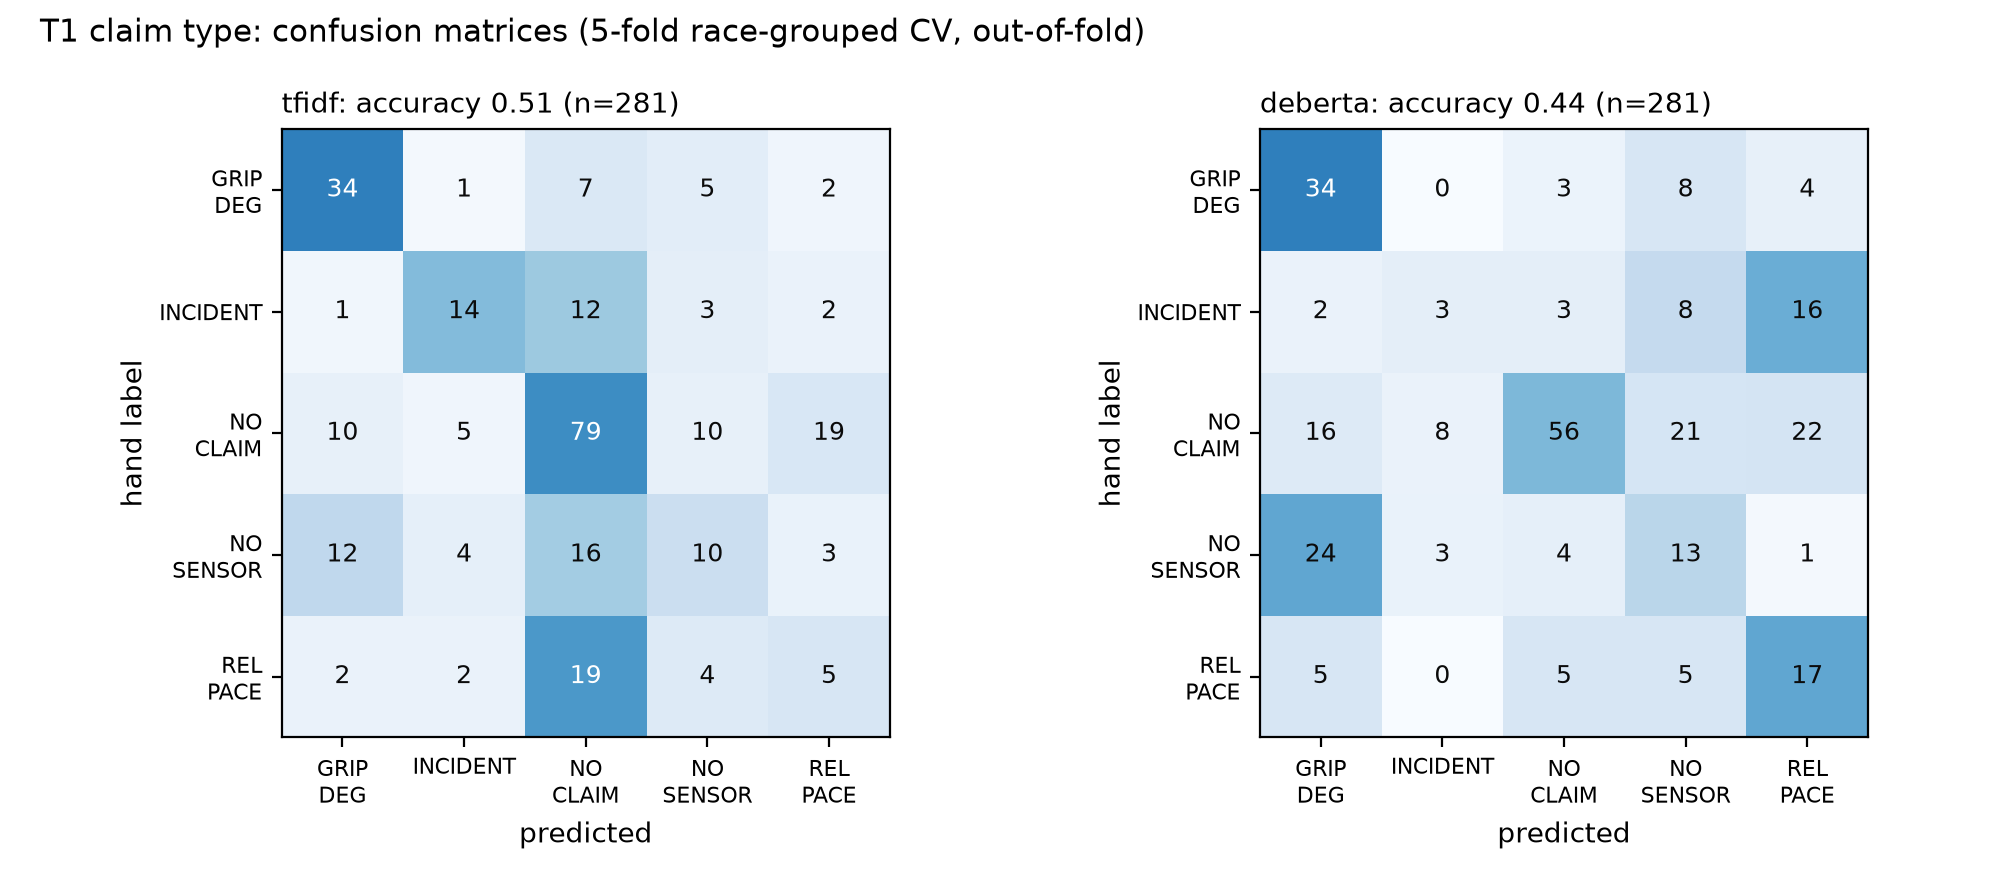
\includegraphics[width=0.85\textwidth]{fig8_confusion.png}
\caption{T1 confusion matrices (out-of-fold, 5-fold race-grouped CV).}
\label{fig:conf}
\end{figure*}

\subsection{Arousal Estimation (T3)}
\emph{Verdict: strong.}

\begin{figure}[t]
\centering
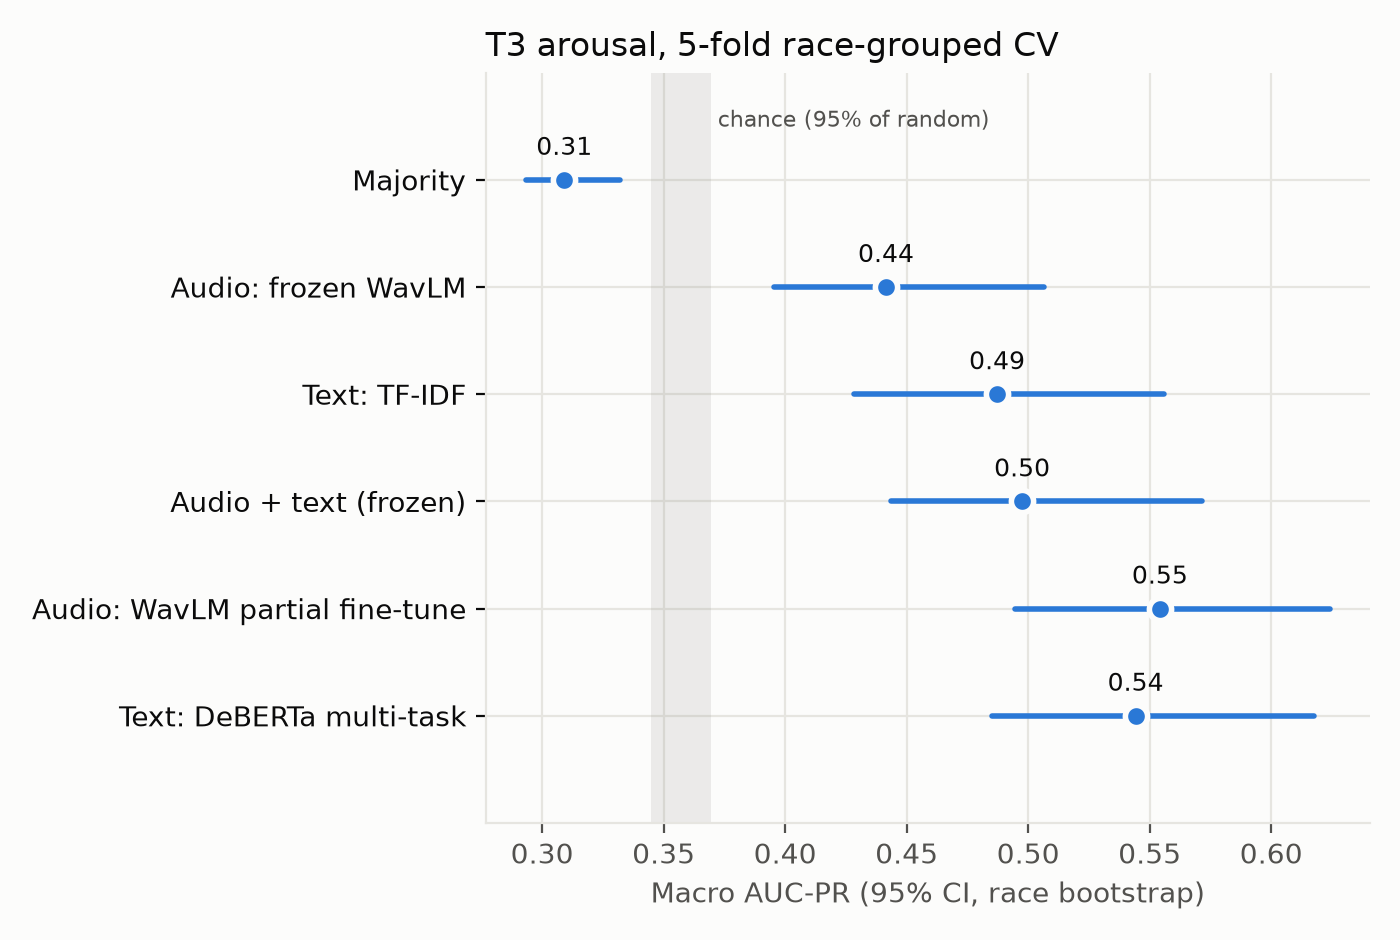
\includegraphics[width=\columnwidth]{fig4_t3_arousal.png}
\caption{T3 arousal, macro AUC-PR (5-fold race-grouped CV, 95\% CI). Partial fine-tuning of WavLM and the multi-task DeBERTa are the strongest models.}
\label{fig:t3}
\end{figure}
With frozen WavLM features plus prosody (z-scored within driver-race), audio reaches 0.442 macro AUC-PR (CI 0.396--0.507), $+0.132$ over majority (CI $+0.080$ to $+0.199$); for high arousal its AUC-PR is about twice chance (0.25 vs.\ 0.12). Stacking audio with text probabilities gives 0.498, better than audio alone ($+0.056$, CI $+0.021$ to $+0.093$) but not than text alone ($+0.010$, CI $-0.067$ to $+0.080$). Text's strength should be read with care: the annotator saw the transcript while judging arousal, so text-based scores may partly reflect cues that shaped the labels.

\textbf{Partial fine-tuning.} Fine-tuning WavLM's upper six layers with a learned layer weighting (lower six frozen) raises audio arousal to \textbf{0.554} macro AUC-PR (CI 0.495--0.624), the best arousal model in the study, ahead of the frozen-feature model (0.442) and on par with the multi-task text model (0.544). The learned weights favour the upper-middle layers (layer 10: 0.182, layer 11: 0.179, against a uniform 0.167), consistent with paralinguistic information concentrating below the top layer. On identical items and folds, the gain from partial fine-tuning over frozen features is $+0.113$ (paired 95\% CI $+0.028$ to $+0.192$). Holding out each of the top eight drivers in turn (crossed with race folds; 188 utterances) gives 0.513 (CI 0.422--0.612; chance 0.349), and the learned layer weights are the same in every fold and protocol, peaking at layers 10--11.

\subsection{Telemetry Consistency: Rules (T2)}
\emph{Verdict: null.}

\begin{table}[t]
\centering
\caption{T2 telemetry-consistency of in-race claims, primary pre-registered thresholds: share of claims for which the rule fires, versus the same car's base rate and the reverse-time placebo (3 laps earlier).}
\label{tab:t2}
\begin{tabular}{lrccc}
\toprule
Claim & $n$ & At claim & Base rate & Placebo \\
\midrule
\textsc{grip\_deg} & 45 & 0.24 & 0.23 & 0.28 \\
\textsc{traffic} & 24 & 0.64 & 0.49 & 0.50 \\
\textsc{rel\_pace} & 30 & 0.80 & 0.87 & 0.80 \\
\textsc{incident} & 30 & 0.11 & 0.05 & 0.10 \\
\textsc{power} & 11 & 0.40 & 0.19 & 0.60 \\
\bottomrule
\end{tabular}
\end{table}
No difference between consistency and the matched base rate excludes zero (Table~\ref{tab:t2}). \textsc{traffic} is the closest to a signal ($+0.15$, CI $-0.04$ to $+0.29$). \textsc{incident} claims coincide with race-control messages twice as often as the base rate, but the placebo is as high, so the event predates the message. This is consistent with radio being broadcast at eventful moments: across all claim types, rules fire more often on radio laps than on the car's other laps. The \textsc{rel\_pace} rule fires on 84\% of all laps and cannot discriminate.

\subsection{Telemetry Consistency: Neural Model (T2)}
\emph{Verdict: null.}

On the 250 in-race labelled claims (classes \textsc{grip\_deg}, \textsc{incident}, \textsc{rel\_pace} and \textsc{other}; chance 0.266, 95th percentile 0.293), the gated cross-attention model reaches 0.312 macro AUC-PR and naive concatenation 0.300; the gated model's advantage ($+0.013$, CI $-0.021$ to $+0.053$) is in the direction reported for constrained fusion~\cite{lee2026cfa} but not significant at this size (Fig.~\ref{fig:t2n}). Neither beats the context-only baseline (0.291; gated $-$ context $+0.021$, CI $-0.024$ to $+0.072$). \textbf{Decisively, the reverse-time placebo scores the same} (0.310; gated $-$ placebo $+0.002$, CI $-0.046$ to $+0.047$). A simple logistic regression on lap tokens edges past context ($+0.055$, CI $0.000$ to $+0.115$) but not past its own placebo ($+0.026$, CI $-0.016$ to $+0.066$): what it detects is slow-moving race state that was already present three laps earlier, not the claimed event.

\begin{figure}[t]
\centering
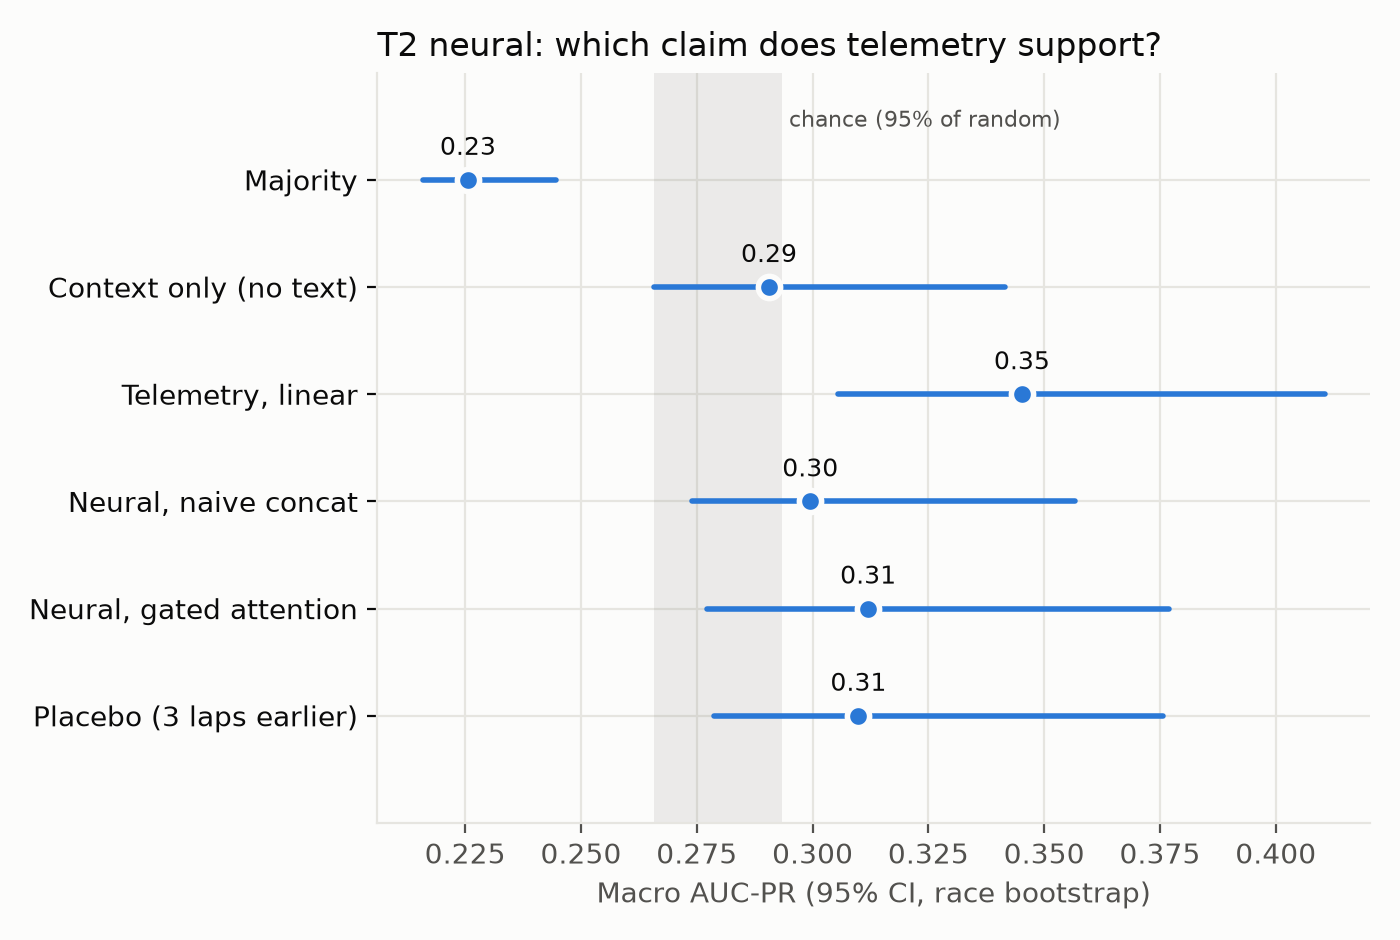
\includegraphics[width=\columnwidth]{fig6_t2_neural.png}
\caption{Neural T2: macro AUC-PR for predicting the human claim label from telemetry alone, with baselines and the reverse-time placebo.}
\label{fig:t2n}
\end{figure}

\subsection{Placebo Control}
Across both T2 analyses the reverse-time placebo matches the real window. Together with the elevated rule rates on radio laps generally, this indicates that broadcast radio is selected at eventful moments: any telemetry signal around a message predates it. Without this control, the \textsc{incident} result and the telemetry-LR result would have been reported as positives.

\subsection{Arousal and Subsequent Laps (T4)}
\emph{Verdict: null.}

Arousal probabilities came from the best T3 model by cross-validated AUC-PR (partial fine-tuned WavLM, 0.554 vs.\ 0.498 for the fused frozen model), a rule fixed before T4 was run. The MDE, written to disk before fitting, is 0.26\,s per lap for the mean residual over the next three laps and 0.27\,s for the residual SD over the next five (Fig.~\ref{fig:t4}). The estimated effect of going from calm to aroused is $+0.147$\,s (slower; 95\% CI $-0.020$ to $+0.315$; $p=0.084$; 1{,}794 laps, 33 drivers) on the mean residual and $-0.020$\,s (CI $-0.118$ to $+0.077$) on variability. Both are below the MDE. The hand-labelled attenuation check does not support even the direction of the first estimate ($-0.005$, CI $-0.193$ to $+0.183$, $n=191$). Random slopes by driver do not improve on random intercepts (likelihood-ratio $p=0.19$ and $0.55$); the slope variance component is 0.051 (SD 0.23\,s) and 0.008. We report a null: arousal effects on subsequent pace smaller than about a quarter of a second per lap cannot be detected with these data. In-race positive affect is rare (cheerful radio is mostly post-race, with no following lap), so the axis studied is arousal versus a calm baseline, not happy versus angry.

\begin{figure}[t]
\centering
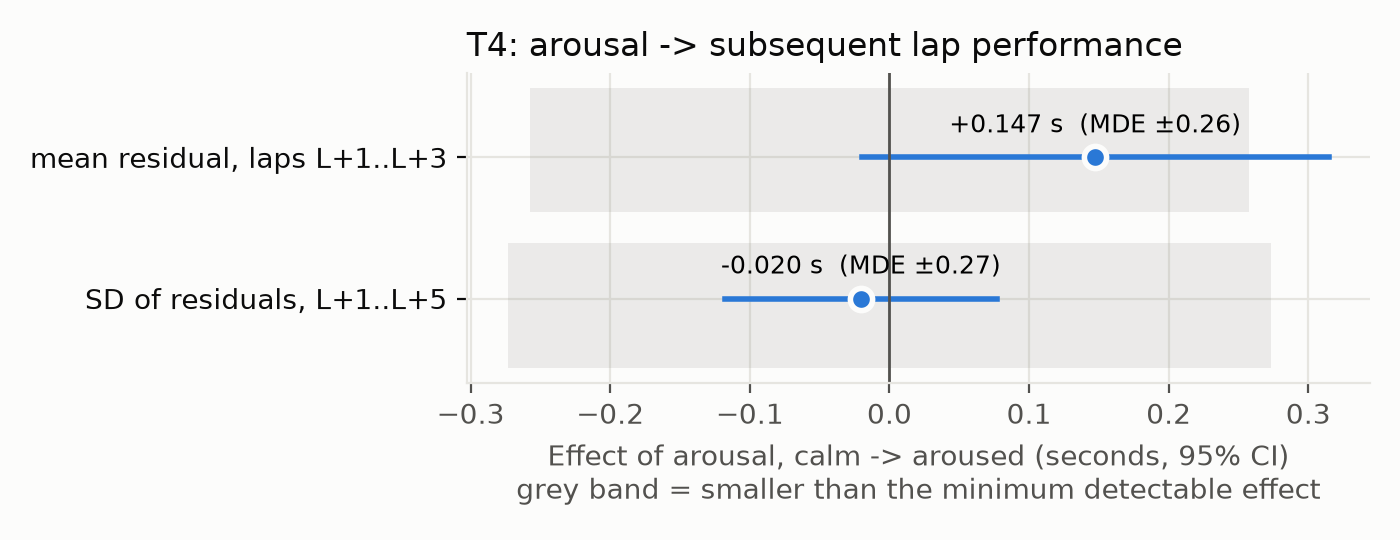
\includegraphics[width=\columnwidth]{fig7_t4.png}
\caption{T4: estimated effect of arousal on subsequent laps (95\% CI) against the minimum detectable effect (grey).}
\label{fig:t4}
\end{figure}

\subsection{Learning Curve}
Because DeBERTa did not beat TF-IDF, we ran the learning curve committed to in advance (Fig.~\ref{fig:lc}): within the same race-grouped folds, training races were subsampled to 25--100\%. DeBERTa improves twice as steeply as TF-IDF (0.272$\rightarrow$0.426 vs.\ 0.390$\rightarrow$0.466 from $\sim$58 to $\sim$225 training examples per fold) and briefly matches it at $\sim$167 examples (0.427 vs.\ 0.422), but flattens at the last step, where the confidence intervals overlap. Fine-tuning gains more from extra labels, but these data give no evidence that it would overtake TF-IDF, let alone the zero-shot LLM (0.629), with modestly more annotation.

\begin{figure}[t]
\centering
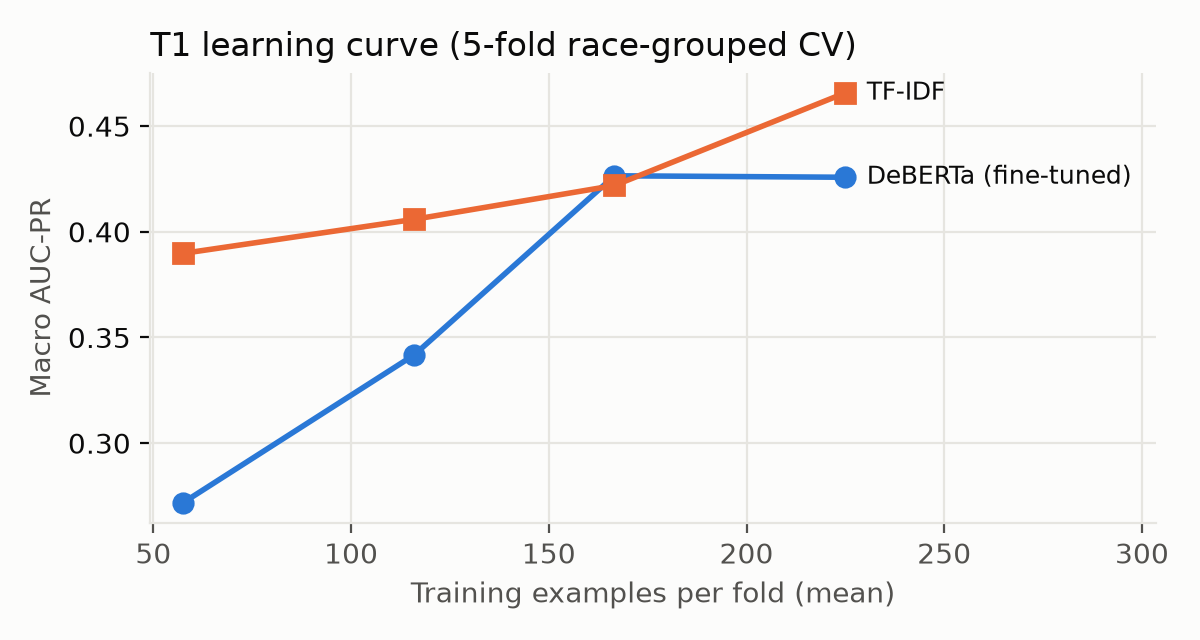
\includegraphics[width=\columnwidth]{fig9_learning_curve.png}
\caption{T1 learning curve: macro AUC-PR versus training examples per fold, 5-fold race-grouped CV.}
\label{fig:lc}
\end{figure}
